\chapter{Análisis}
\label{cap:analisis}

\section{Introducción al problema}

Nos encontramos ante la siguiente situación: Debemos permitir al usuario realizar consultas sobre las imágenes de su dispositivo, tomando como imagen consulta la obtenida desde la cámara o desde la galería.\\

Los valores proporcionados por cada descriptor se encuentran en el rango 0-1. Los cálculos para determinar la posición se realizarán con esos datos. Para ello, se colocarán de izquierda a derecha, formando un total de 4 columnas, siguiendo un orden lógico y natural que es entendido rápida y claramente por el usuario.\\

Dado el número de imágenes y el tamaño de pantalla de los dispositivos, no todas podrán ser vistas a la vez ni, por lo que el usuario debe ser capaz de desplazarse por las imágenes resultado contando con guı́as que le indiquen el orden de las diferentes imágenes mostradas.\\

También deberá ser posible obtener información de las imágenes mostradas con el fin de comprender mejor la visualización y su vez comprobar el correcto funcionamiento de los descriptores.\\

El proyecto está pensado por el momento sólo para smartphones, debido a falta de medios, por lo que la posibilidad de girar pantalla ha sido desactivada. Como trabajo futuro, se realizarán los cambios oportunos para que pueda ser utilizado en tablets.

\section{Especificación de requisitos}

Por requisitos podemos entender: Condición o capacidad que necesita el usuario para resolver un problema o conseguir un objetivo determinado.\\

Como en todo proyecto de software, los requisitos deben ser especificados antes de empezar el desarrollo del mismo.\\

En esta sección vamos a detallar cada uno de los distintos requisitos necesitados agrupados en requisitos funcionales, no funcionales y de información.\\

\subsection{Requisitos funcionales}

Los requisitos funcionales se encargan de especificar cómo se realizará la interacción entre el sistema y su entorno, indicando los servicios que ha de tener el sistema o cómo responderá ante ciertos estímulos.\\

Este proyecto cuenta con los siguientes requisitos funcionales:\\

\textbf{RF-1. Imágenes:} Gestión de imágenes.\\
 
   RF-1.1. Se debe permitir cargar cualquier imagen desde cámara o galería como imagen consulta.
   
   RF-1.2. Se debe permitir cargar cualquier número de imágenes para su consulta.
   
   RF-1.3. La elección de la imagen consulta ha de ser sencilla.\\
   
\textbf{RF-2. Descriptores:} Gestión de descriptores.\\    
   
   RF-2.1. Ha de ser posible la elección de cualquier descriptor disponible.
      
   RF-2.2. La consulta ha de realizarse con únicamente con el descriptor seleccionado.\\    
   
\textbf{RF-3. Base de datos:} Gestión de base de datos.\\    
   
   RF-3.1. El usuario debe poder precalcular la base de datos antes de realizar cualquier consulta.
   
   RF-3.2. El usuario debe poder eliminar la base de datos, en caso de que lo considere necesario.\\

\textbf{RF-4 Interacción} Gestión de la interacción.\\

   RF-4.1. El usuario debe poder interactuar a través de la pantalla.
   
   RF-4.2. El usuario debe ser capaz de desplazar las imágenes consulta de izquierda a derecha y viceversa.
   
   RF-4.3. El usuario debe ser capaz de desplazar las imágenes resultado de arriba hacia abajo y viceversa.
   
   RF-4.4. El usuario debe poder ver las imágenes a tamaño real al pulsar sobre ellas.

\textbf{RF-5 Información adicional} Gestión de la información adicional.\\

   RF-5.1. El usuario debe poder consultar información sobre el desarrollo del proyecto.
   
   RF-5.2. El usuario debe ser capaz de obtener más información sobre sistemas de recuperación de imágenes y sobre los descriptores.
   
           
\subsection{Requisitos no funcionales}
Los requisitos no funcionales describen cualidades o restricciones del sistema que no se relacionan de forma directa con el comportamiento funcional del mismo.

Este proyecto cuenta con los siguientes requisitos no funcionales:\\

\textbf{RNF-1} Debe de utilizar la mínima cantidad de memoria posible.

\textbf{RNF-2} Ha de ser implementando en Android.

\textbf{RNF-3} Ha de requerir los permisos mínimos para funcionar.

\textbf{RNF-4} Las consultas se realizan utilizando una única imagen consulta.
   
\textbf{RNF-5} El tamaño de las imágenes mostradas ha de ser lo suficientemente grande para poder verse correctamente.

\textbf{RNF-6} Se debe indicar el orden en el que fueron dibujadas las imágenes.\\

\subsection{Requisitos de información}

Este tipo de requisito de detallar la necesidad por parte del sistema del almacenamiento de la información. \\

\textbf{RI-1} Almacenar información de la consulta para evitar nuevas cálculos innecesarias.


\section{Historias de usuario}

Cuando nos referimos a historias de usuario, nos referiremos a la representación de un requisito software que se encuentra escrito en varias frases cortas, utilizando el lenguaje común del usuario. Esto facilita la comprensión y realización de los requisitos de un proyecto. Se trata de otra manera de ver los requisitos software que se acaban de explicar. Por lo que vamos a ver sólo los principales\\

\begin{table}[H]
	\begin{center}
		\begin{tabular} {l|c|l}
			\hline
			1 & \multicolumn{2}{c}{Interacción con la interfaz} \\ \noalign{\hrule height 1pt}
			\multicolumn{3}{l}{Descripción} \\ \hline
			\multicolumn{3}{p{12cm}}{Se podrá mover con libertad por los distintos menús disponibles en la interfaz.} \\ \noalign{\hrule height 1pt}
			\multicolumn{3}{l}{Pruebas de aceptación} \\ \hline
			\multicolumn{3}{p{12cm}}{ - Comprobar que al pulsar en al pulsar el ítem \textbf{consulta} se muestra la interfaz asociada.} \\
			\multicolumn{3}{p{12cm}}{ - Comprobar que al pulsar en el action button, este se despliega mostrando dos opciones, cámara y galería.} \\
			\multicolumn{3}{p{12cm}}{ - Comprobar que al pulsar en al pulsar el ítem \textbf{ajustes} se muestra la interfaz asociada.} \\ \hline
			\multicolumn{3}{p{12cm}}{ - Comprobar que al pulsar en al pulsar el ítem \textbf{adicional} se muestra la interfaz asociada.} \\ 
			\hline
		\end{tabular}
	\end{center}
	\caption{Historia de usuario - Interacción con la interfaz}
	\label{tab:interaccion-interfaz}
\end{table}

\begin{table}[H]
	\begin{center}
		\begin{tabular} {l|c|l}
			\hline
			2 & \multicolumn{2}{c}{Cargar imagen cámara} \\ \noalign{\hrule height 1pt}
			\multicolumn{3}{l}{Descripción} \\ \hline
			\multicolumn{3}{p{12cm}}{Se podra mover cargar la imagen consulta utilizando la cámara del dispositivo.} \\ \noalign{\hrule height 1pt}
			\multicolumn{3}{l}{Pruebas de aceptación} \\ \hline
			\multicolumn{3}{p{12cm}}{ - Comprobar que al pulsar en al pulsar el ítem \textbf{cámara} del \textit{floating button}, se lanza la actividad cámara, pudiendo elegir la delantera o trasera en caso de que se disponga de ellas.} \\
			\multicolumn{3}{p{12cm}}{ - Comprobar que al tomar una fotografía esta se añade a la sección de imágenes consulta.} \\
			\multicolumn{3}{p{12cm}}{ - Comprobar que al pulsar en al pulsar en el ítem \textbf{consultar}, se realiza la consulta con esta nueva imagen.} \\ \hline
		\end{tabular}
	\end{center}
	\caption{Historia de usuario - Cargar imagen consulta cámara}
	\label{tab:interaccion-interfaz}
\end{table}

\begin{table}[H]
	\begin{center}
		\begin{tabular} {l|c|l}
			\hline
			3 & \multicolumn{2}{c}{Cargar imagen galería} \\ \noalign{\hrule height 1pt}
			\multicolumn{3}{l}{Descripción} \\ \hline
			\multicolumn{3}{p{12cm}}{Se podrá cargar la imagen consulta utilizando la galería del dispositivo.} \\ \noalign{\hrule height 1pt}
			\multicolumn{3}{l}{Pruebas de aceptación} \\ \hline
			\multicolumn{3}{p{12cm}}{ - Comprobar que al pulsar en al pulsar el ítem \textbf{galería} del \textit{floating button}, se lanza la galería.} \\
			\multicolumn{3}{p{12cm}}{ - Comprobar que al tomar seleccionar una imagen, esta se añade a la sección de imágenes consulta.} \\
			\multicolumn{3}{p{12cm}}{ - Comprobar que al pulsar en al pulsar en el ítem \textbf{consultar}, se realiza la consulta con esta nueva imagen.} \\ \hline
		\end{tabular}
	\end{center}
	\caption{Historia de usuario - Cargar imagen consulta galería}
	\label{tab:interaccion-interfaz}
\end{table}


\begin{table}[H]
	\begin{center}
		\begin{tabular} {l|c|l}
			\hline
			4 & \multicolumn{2}{c}{Cambiar de descriptor} \\ \noalign{\hrule height 1pt}
			\multicolumn{3}{l}{Descripción} \\ \hline
			\multicolumn{3}{p{12cm}}{Se podrá cambiar el descriptor que se emplea durante las consultas.} \\ \noalign{\hrule height 1pt}
			\multicolumn{3}{l}{Pruebas de aceptación} \\ \hline
			\multicolumn{3}{p{12cm}}{ - Comprobar que al pulsar sobre el descriptor deseado este queda marcado como activo.} \\
			\multicolumn{3}{p{12cm}}{ - Comprobar que solo un descriptor puede ser seleccionado.} \\
			\multicolumn{3}{p{12cm}}{ - Comprobar que al pulsar en al pulsar en el ítem \textbf{consultar}, se realiza la consulta con este descriptor seleccionado.} \\ \hline
		\end{tabular}
	\end{center}
	\caption{Historia de usuario - Cambiar descriptor}
	\label{tab:interaccion-interfaz}
\end{table}

\begin{table}[H]
	\begin{center}
		\begin{tabular} {l|c|l}
			\hline
			5 & \multicolumn{2}{c}{Eliminar base de datos} \\ \noalign{\hrule height 1pt}
			\multicolumn{3}{l}{Descripción} \\ \hline
			\multicolumn{3}{p{12cm}}{Se podrá eliminar la base de datos.} \\ \noalign{\hrule height 1pt}
			\multicolumn{3}{l}{Pruebas de aceptación} \\ \hline
			\multicolumn{3}{p{12cm}}{ - Comprobar que al pulsar sobre la opción \textit{Eliminar BD} se lanza un desplegable para realizar la acción.} \\
			\multicolumn{3}{p{12cm}}{ - Comprobar que al pulsar en aceptar, se notifica de que la BD ha sido eliminada.} \\
		\end{tabular}
	\end{center}
	\caption{Historia de usuario - Eliminar base de datos}
	\label{tab:interaccion-interfaz}
\end{table}

\begin{table}[H]
	\begin{center}
		\begin{tabular} {l|c|l}
			\hline
			6 & \multicolumn{2}{c}{Calcular base de datos} \\ \noalign{\hrule height 1pt}
			\multicolumn{3}{l}{Descripción} \\ \hline
			\multicolumn{3}{p{12cm}}{Se podrá precalcular la base de datos para agilizar consultas.} \\ \noalign{\hrule height 1pt}
			\multicolumn{3}{l}{Pruebas de aceptación} \\ \hline
			\multicolumn{3}{p{12cm}}{ - Comprobar que al pulsar sobre la opción \textit{Calcular BD} se lanza un diálogo sobre el proceso.} \\
			\multicolumn{3}{p{12cm}}{ - Comprobar que al realizar una consulta, el tiempo es menor que si no hubiese base de datos.} \\
		\end{tabular}
	\end{center}
	\caption{Historia de usuario - Calcular base de datos}
	\label{tab:interaccion-interfaz}
\end{table}

\begin{table}[H]
	\begin{center}
		\begin{tabular} {l|c|l}
			\hline
			7 & \multicolumn{2}{c}{Elegir número de imágenes} \\ \noalign{\hrule height 1pt}
			\multicolumn{3}{l}{Descripción} \\ \hline
			\multicolumn{3}{p{12cm}}{Se podrá elegir el número de imágenes que serán consultadas.} \\ \noalign{\hrule height 1pt}
			\multicolumn{3}{l}{Pruebas de aceptación} \\ \hline
			\multicolumn{3}{p{12cm}}{ - Comprobar que al pulsar sobre la opción \textit{Elegir número de imágenes} se lanza un desplegable permitiendonos elegir el número.} \\
			\multicolumn{3}{p{12cm}}{ - Comprobar que el número de las imágenes resultado se corresponde con el establecido previamente.} \\
		\end{tabular}
	\end{center}
	\caption{Historia de usuario - Elegir número de imágenes}
	\label{tab:interaccion-interfaz}
\end{table}

\begin{table}[H]
	\begin{center}
		\begin{tabular} {l|c|l}
			\hline
			8 & \multicolumn{2}{c}{Interactuar con las imágenes consulta} \\ \noalign{\hrule height 1pt}
			\multicolumn{3}{l}{Descripción} \\ \hline
			\multicolumn{3}{p{12cm}}{Se podrá interactuar con las imágenes consulta.} \\ \noalign{\hrule height 1pt}
			\multicolumn{3}{l}{Pruebas de aceptación} \\ \hline
			\multicolumn{3}{p{12cm}}{ - Comprobar que se puede realizar movimiento scroll de derecha a izquierda y viceversa sobre las imágenes consulta, siempre que haya las suficientes.} \\
			\multicolumn{3}{p{12cm}}{ - Comprobar que al pulsar sobre una, esta se muestra a pantalla completa indicándonos la posición que ocupa respecto a las demás.} \\
		\end{tabular}
	\end{center}
	\caption{Historia de usuario - Interactuar con las imágenes consulta }
	\label{tab:interaccion-interfaz}
\end{table}

\begin{table}[H]
	\begin{center}
		\begin{tabular} {l|c|l}
			\hline
			9 & \multicolumn{2}{c}{Interactuar con las imágenes resultado} \\ \noalign{\hrule height 1pt}
			\multicolumn{3}{l}{Descripción} \\ \hline
			\multicolumn{3}{p{12cm}}{Se podrá interactuar con las imágenes resultado.} \\ \noalign{\hrule height 1pt}
			\multicolumn{3}{l}{Pruebas de aceptación} \\ \hline
			\multicolumn{3}{p{12cm}}{ - Comprobar que se puede realizar movimiento scroll hacia arriba, hacia abajo y viceversa sobre las imágenes resultado, siempre que haya las suficientes.} \\
			\multicolumn{3}{p{12cm}}{ - Comprobar que al pulsar sobre una, esta se muestra a pantalla completa indicándonos la posición que ocupa respecto a las demás, y la distancia respecto a la imagen consulta.} \\
		\end{tabular}
	\end{center}
	\caption{Historia de usuario - Interactuar con las imágenes consulta}
	\label{tab:interaccion-interfaz}
\end{table}

\section{Diagramas de secuencia}

Establecidas las historias de usuario, procedamos con los diagramas de secuencia. Estos se usan para establecer el modo en que interaccionan objetos en un sistema atendiendo a UML.

\begin{figure}[H] %con el [H] le obligamos a situar aquí la figura
\centering
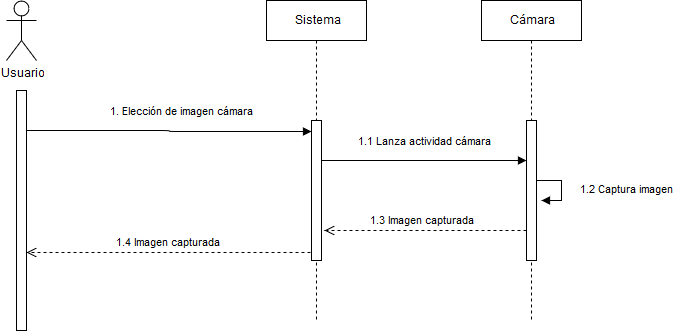
\includegraphics[scale=0.6]{imagenes/imagenCamara.png}  %el parámetro scale permite agrandar o achicar la imagen. En el nombre de archivo puede especificar directorios
\label{imagenCamara.png}
\caption{Diagrama de secuencia imagen consulta cámara}
\end{figure}

\begin{figure}[H] %con el [H] le obligamos a situar aquí la figura
\centering
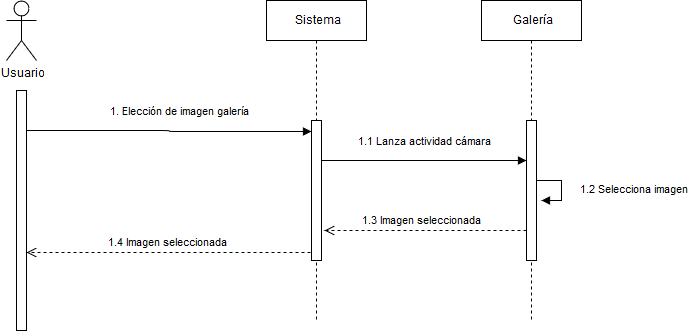
\includegraphics[scale=0.6]{imagenes/imagenGaleria.png}  %el parámetro scale permite agrandar o achicar la imagen. En el nombre de archivo puede especificar directorios
\label{imagenGaleria.png}
\caption{Diagrama de secuencia imagen consulta galería}
\end{figure}

\begin{figure}[H] %con el [H] le obligamos a situar aquí la figura
\centering
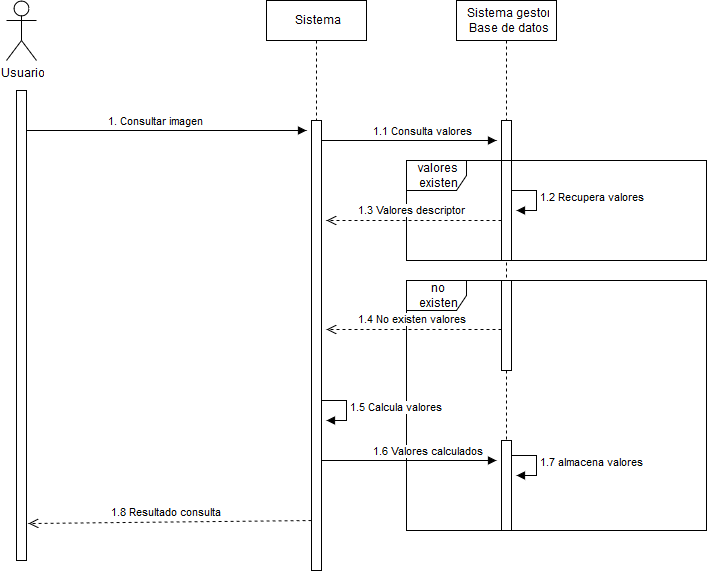
\includegraphics[scale=0.6]{imagenes/realizarConsulta.png}  %el parámetro scale permite agrandar o achicar la imagen. En el nombre de archivo puede especificar directorios
\label{realizarConsulta.png}
\caption{Diagrama de secuencia imagen realizar consulta}
\end{figure}

\begin{figure}[H] %con el [H] le obligamos a situar aquí la figura
\centering
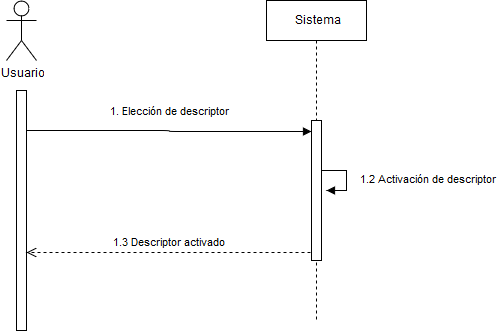
\includegraphics[scale=0.6]{imagenes/eleccionDescriptor.png}  %el parámetro scale permite agrandar o achicar la imagen. En el nombre de archivo puede especificar directorios
\label{realizarConsulta.png}
\caption{Diagrama de secuencia elección descriptor}
\end{figure}

\begin{figure}[H] %con el [H] le obligamos a situar aquí la figura
\centering
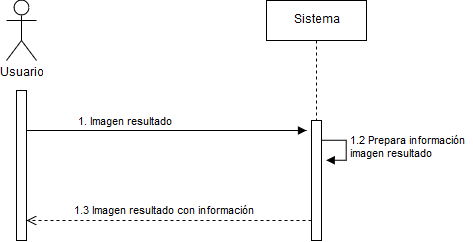
\includegraphics[scale=0.6]{imagenes/imagenResultadoInformacion.png}  %el parámetro scale permite agrandar o achicar la imagen. En el nombre de archivo puede especificar directorios
\label{imagenResultadoInformacion.png}
\caption{Diagrama de secuencia información imagen resultado}
\end{figure}

\begin{figure}[H] %con el [H] le obligamos a situar aquí la figura
\centering
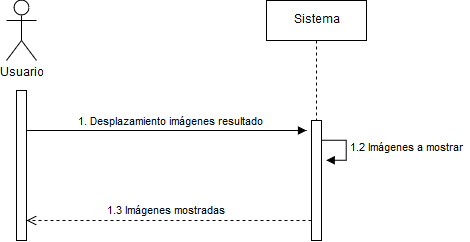
\includegraphics[scale=0.6]{imagenes/desplazamientoResultado.png}  %el parámetro scale permite agrandar o achicar la imagen. En el nombre de archivo puede especificar directorios
\label{desplazamientoResultado.png}
\caption{Diagrama de secuencia desplazamiento imagen resultado}
\end{figure}

\begin{figure}[H] %con el [H] le obligamos a situar aquí la figura
\centering
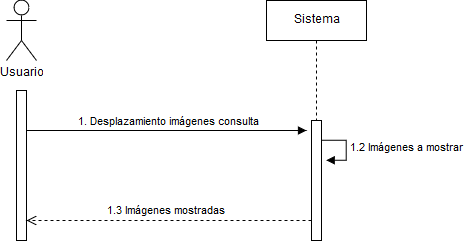
\includegraphics[scale=0.6]{imagenes/desplazamientoConsulta.png}  %el parámetro scale permite agrandar o achicar la imagen. En el nombre de archivo puede especificar directorios
\label{desplazamientoConsulta.png}
\caption{Diagrama de secuencia desplazamiento imagen consulta}
\end{figure}



